\documentclass[10pt]{article}
\usepackage{amsmath,amssymb}
\usepackage[margin=1.5in]{geometry}
\usepackage[colorlinks,citecolor=magenta]{hyperref}
\usepackage{mathtools}
\usepackage{float}
\usepackage[margin=1cm]{caption}

\usepackage{fancyhdr}
\pagestyle{fancy}
\fancyhead{}
\fancyfoot{}
\fancyhead[CO]{\textsc{\small Source, Hess-Smith, and Basu-Hancock Panel Methods}}
\fancyfoot[L]{\href{http://mikef.org}{\emph{\small Michael J. Fairchild}}}
\fancyfoot[R]{\emph{\small Princeton University}}

\DeclarePairedDelimiter\abs{\lvert}{\rvert}
\newcommand\figref[1]{Figure \ref{#1}}
\newcommand\defn[1]{\emph{#1}}
\newcommand\pd[2]{\frac{\partial{#1}}{\partial{#2}}}
\def\eg{e.g.~}
\def\ie{i.e.~}

\begin{document}

\section{Introduction}
The aim of this document is to explain three basic panel methods for the flow of an inviscid, incompressible, two-dimensional fluid past an immersed body: the source panel method for steady nonlifting flows, the Hess-Smith method \cite{hess-smith} for steady lifting flows, and the Basu-Hancock method \cite{basu-hancock} for unsteady lifting flows.  The basic idea of a panel method is to construct the solution as a superposition of certain elementary solutions, with the weights in the linear combination chosen to satisfy appropriate boundary conditions.  For the problems considered here, the fluid region $\Omega\subset\mathbb R^2$ is assumed to be \defn{periphractic}, \ie externally unbounded but internally bounded by one or more simple closed curves.  The equations to be solved are the Euler equations
\begin{equation}\label{eqn:euler}
\pd{\mathbf u}{t}+(\mathbf u\cdot\nabla)\mathbf u = -\frac{1}{\rho}\nabla p\quad,\quad\nabla\cdot{\mathbf u}=0,
\end{equation}
for the flow field $\mathbf u$ in $\Omega$, where $\rho$ is the density and $p$ the pressure, subject to the \defn{flow tangency} boundary condition that $\mathbf u$ be parallel to the boundary $\partial\Omega$.  The elementary solutions we superpose are those of a unit-strength point source at the origin and that of a unit-strength point vortex at the origin, the flows $\mathbf u_s$ and $\mathbf u_v$ of which are given in Cartesian $(x,y)$ coordinates by \[\mathbf u_s(x,y) = \frac{1}{2\pi}\left(\frac{x}{x^2+y^2},\frac{y}{x^2+y^2}\right)\quad,\quad\mathbf u_v(x,y) = \frac{1}{2\pi}\left(\frac{-y}{x^2+y^2},\frac{x}{x^2+y^2}\right).\]  Of course, for a point source or point vortex located at $(x_0,y_0)$, the flow is given by the above equations but with the substitutions $x\mapsto x-x_0$ and $y\mapsto y-y_0$.  (One may object that $\mathbf u_s$ is not divergence free, as required by \eqref{eqn:euler}, but we will place sources only along the boundary of the flow region, and so the flow region itself will be divergence free.)

Each of the three panel methods is implemented in the accompanying code.  The author found the thesis by Teng \cite{teng-thesis} to be particularly valuable in understanding the Basu-Hancock method.

\section{Source-panel method}
Suppose we immerse the unit cylinder into the steady (\ie not varying with time) \defn{onset flow} $\mathbf u_\infty$.  To find the resulting flow, we partition the boundary of the cylinder into a sequence of straight-line panels, say $P_1,\ldots,P_N$, starting at unity and proceeding counterclockwise around the cylinder as in \figref{fig:cylinder_panels}.
\begin{figure}[htbp]
\begin{center}
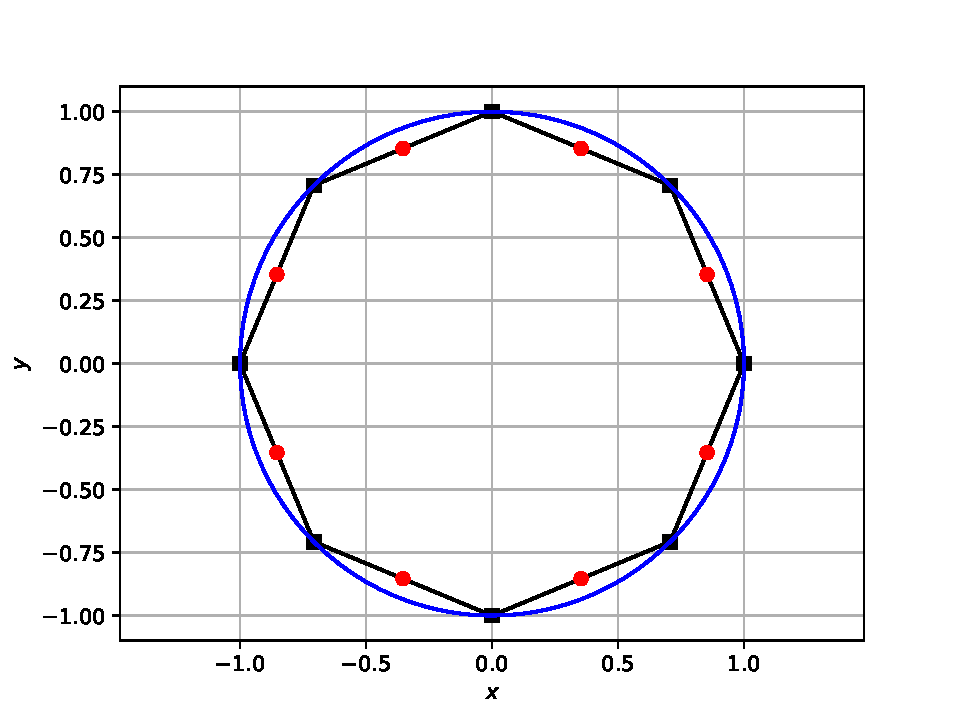
\includegraphics[scale=.5]{plots/cylinder_panels.pdf}
\caption{Approximation of the boundary of the unit cylinder (blue) by a sequence of $N=8$ straight-line panels (black segments).  Each panel has two corner points (black squares) and a midpoint (red dot).}\label{fig:cylinder_panels}
\end{center}
\end{figure}
Each panel $P_i$ is characterized by its two \defn{corner points}, $(x_i,y_i)$ and $(x_{i+1},y_{i+1})$.  Along each panel we distribute a continuous sheet of sources, letting $\sigma_i$ denote the source strength per unit length along panel $P_i$.  The problem is to determine the $N$ unknown scalars $\sigma_1,\ldots,\sigma_N$ such that the resulting flow is tangent to the boundary at $N$ \defn{control points}, which we take to be the midpoints of the panels.

To express the flow-tangency boundary conditions, define the $N\times N$ \defn{influence matrix} $A^n$ such that the $i,j$ entry $A_{ij}^n$, called an \defn{influence coefficient}, denotes the projection along $\hat{\mathbf n}_i$ of the velocity induced at the $i$th control point due to a unit-strength source distribution along the $j$th panel.  Each entry $A_{ij}^n$ of the influence matrix is determined by a line integral treated in the appendix.  The condition that the flow is tangent to the $i$th control point is therefore expressed by the equation \[A_{i1}^n\sigma_1 + \cdots + A_{iN}^n\sigma_N + \mathbf u_\infty\cdot\hat{\mathbf n}_i = 0.\]  There is one such equation for each panel, giving a system of $N$ linear equations in the $N$ unknown strengths $\sigma_1,\ldots,\sigma_N$.  These equations may be arranged into matrix-vector form: \[\begin{bmatrix}A_{11}^n &\cdots &A_{1N}^n\\\vdots &\ddots &\vdots\\A_{N1}^n &\cdots &A_{NN}^n\end{bmatrix}\begin{bmatrix}\sigma_1\\\vdots\\\sigma_N\end{bmatrix}=-\begin{bmatrix}\mathbf u_\infty\cdot\hat{\mathbf n}_1\\\vdots\\\mathbf u_\infty\cdot\hat{\mathbf n}_N\end{bmatrix}.\]  After solving these equations (\eg with Gaussian elimination), we wish to compute the forces on the cylinder.  The forces are due solely to the pressure distribution, which may be found using the \defn{steady Bernoulli equation}, which states that with $q:=\abs{\mathbf u}$,
\begin{equation}\label{eqn:bernoulli_steady}
\frac{1}{2}q^2+\frac{p}{\rho}=\text{constant along a streamline}.
\end{equation}
In particular, $\frac{1}{2}q^2+\frac{p}{\rho}=\frac{1}{2}q_\infty^2+\frac{p_\infty}{\rho}$, where the subscripts on the right side denotes a point far upstream of the cylinder.  The nondimensional \defn{pressure coefficient} $C_p$ encodes the pressure surfeit over the pressure at infinity, measured in multiples of the \defn{dynamic pressure} $\frac{1}{2}\rho q_\infty^2$ (\ie kinetic energy per unit volume of the flow at infinity), and is defined by
\begin{equation}\label{eqn:pressure_coefficient}
C_p:=\frac{p-p_\infty}{\frac{1}{2}\rho q_\infty^2}=1-\left(\frac{q}{q_\infty}\right)^2.
\end{equation}
Hence to compute the pressure distribution around the cylinder, we need only know the net flow speed at points around the cylinder.  Since the source strengths have already been determined, the flow can be computed everywhere; in particular, along the cylinder's boundary.  Indeed, define the $N\times N$ influence matrix $A^t$ such that $A_{ij}^t$ is the projection along $\hat{\mathbf t}_i$ of the velocity at the $i$th control point due to a unit-strength source sheet along the $j$th panel.  Since the flow is tangent to the cylinder, it follows that flow speed $q_i$ at the $i$th control point is \[q_i = A_{i1}^t\sigma_1 + \cdots + A_{iN}^t\sigma_N + \mathbf u_\infty\cdot\hat{\mathbf t}_i.\]  The exact pressure distribution around the cylinder is shown in \cite{currie} to be \[C_p=1-4\sin^2\theta,\] where $\theta$ measures the angle around the cylinder.  The results of the source panel method, with $N=50$ panels, for steady flow past the unit cylinder are displayed in \figref{fig:cylinder_ubem2d}.

The solution to the steady flow problem past a cylinder is not unique, since a point vortex of arbitrary strength may be placed at the center of the cylinder (because the flow due to such a vortex satisfies \eqref{eqn:euler} and is tangent to the cylinder's boundary).  However, for a fixed circulation $\Gamma$ around the cylinder, there is a unique solution, given in \cite{currie} by \[C_p = 1-\left(\frac{\frac{\Gamma}{2\pi}-2q_\infty\sin\theta}{q_\infty}\right)^2,\] which reduces to the previous display when $\Gamma=0$.  The results shown in \figref{fig:cylinder_ubem2d} are for the case of zero ciruclation.

\begin{figure}[H]
\begin{center}
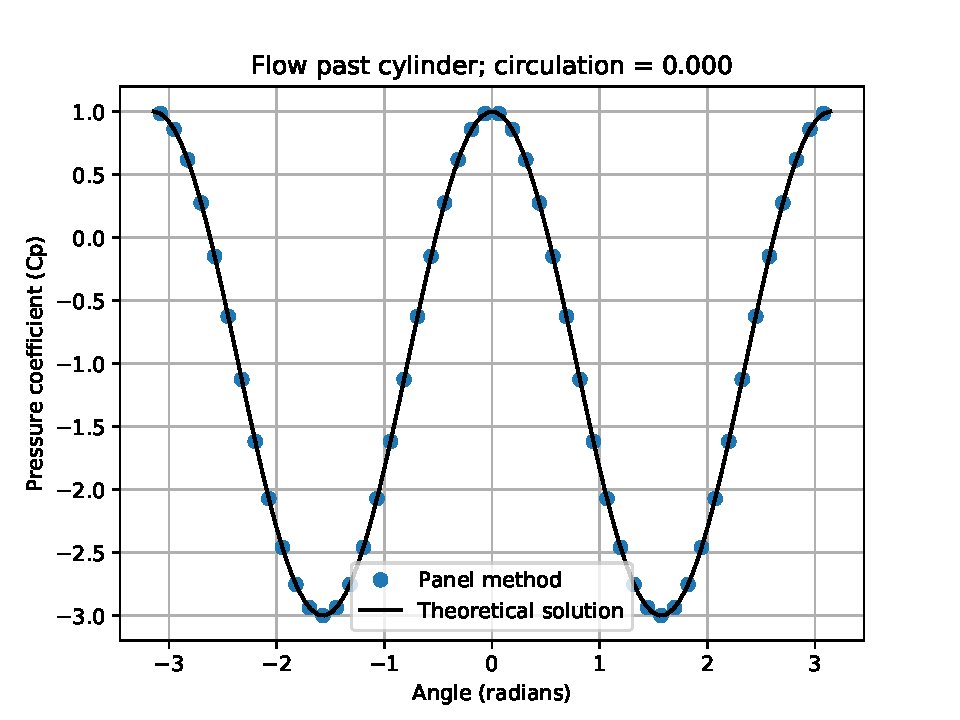
\includegraphics[scale=.4]{plots/cylinder_cp_boundary.pdf}
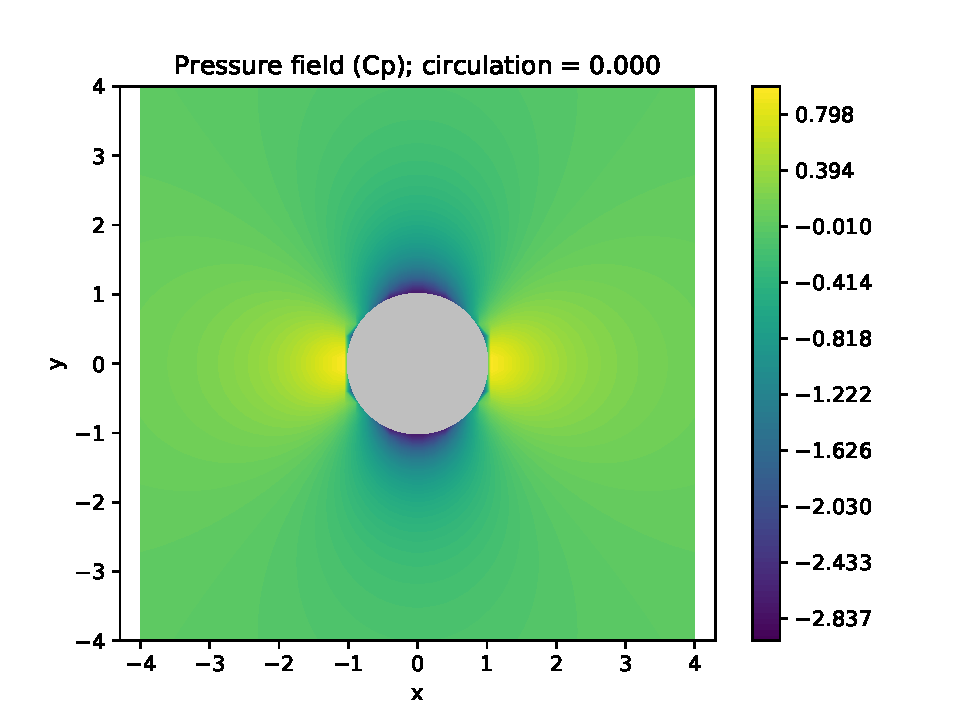
\includegraphics[scale=.4]{plots/cylinder_cp_field.pdf}
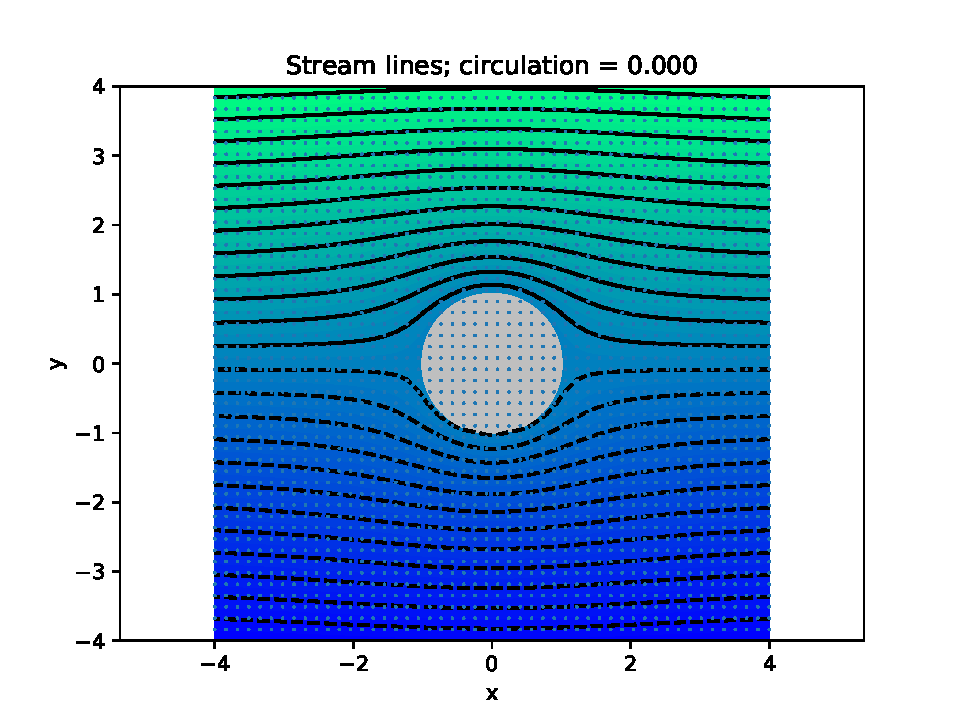
\includegraphics[scale=.4]{plots/cylinder_stream_lines.pdf}
\caption{Results of the source panel method for steady flow $\mathbf u_\infty=\hat{\mathbf x}$ past the unit cylinder.  The pressure coefficient $C_p$ is plotted around the boundary (upper left) and in the flow region (upper right).  The flow streamlines are shown at bottom.}\label{fig:cylinder_ubem2d}
\end{center}
\end{figure}

\section{Hess-Smith method}
We now consider the steady flow past an airfoil with a sharp trailing edge.  Unlike steady flow past a cylinder, which admits infinitely many solutions, experience has shown that when such an airfoil is only slightly inclined to the flow (say, no more than 10 to 15 degrees), then the flow is uniquely determined by the condition that it smoothly detaches from the trailing edge of the airfoil.  One way of formulating this observation is to assert there is no load, \ie pressure difference, at the trailing edge of the airfoil.  This is known as a \defn{Kutta condition}, the mathematical effect of which is to fix the value of circulation around the airfoil.  As emphasized in \cite{basu-hancock}, there is generally no such thing as ``the'' Kutta condition; rather, which condition is needed to obtain a unique and physically meaningful solution depends on problem at hand.  For the rest of this section, our problem is to solve the Euler equations \eqref{eqn:euler} subject to flow tangency boundary conditions and the additional stipulation of no load at the airfoil's trailing edge.  

We will do this using the panel method of Hess and Smith \cite{hess-smith}, which builds upon the source-panel method of the previous section.  As before, the airfoil's boundary is partitioned into a sequence of panels, whose corners we order from the trailing edge to the leading edge along the upper surface and then back to the trailing edge along the lower surface.  Source sheets are placed along each panel, in order to satisfy flow tangency, but now we need an additional unknown in order to satisfy the Kutta condition.  We therefore assume that the airfoil's bondary also has a vortex sheet, of circulation $\gamma$ per unit length, along its boundary.  Unlike the source strengths, which vary from panel to panel, the unknown $\gamma$ is the same for all panels.  The $N+1$ unknowns $\sigma_1,\ldots,\sigma_N,\gamma$ will be determined by $N+1$ equations: $N$ flow tangency equations, and one Kutta condition.

%\begin{figure}[htbp]
%\begin{center}
%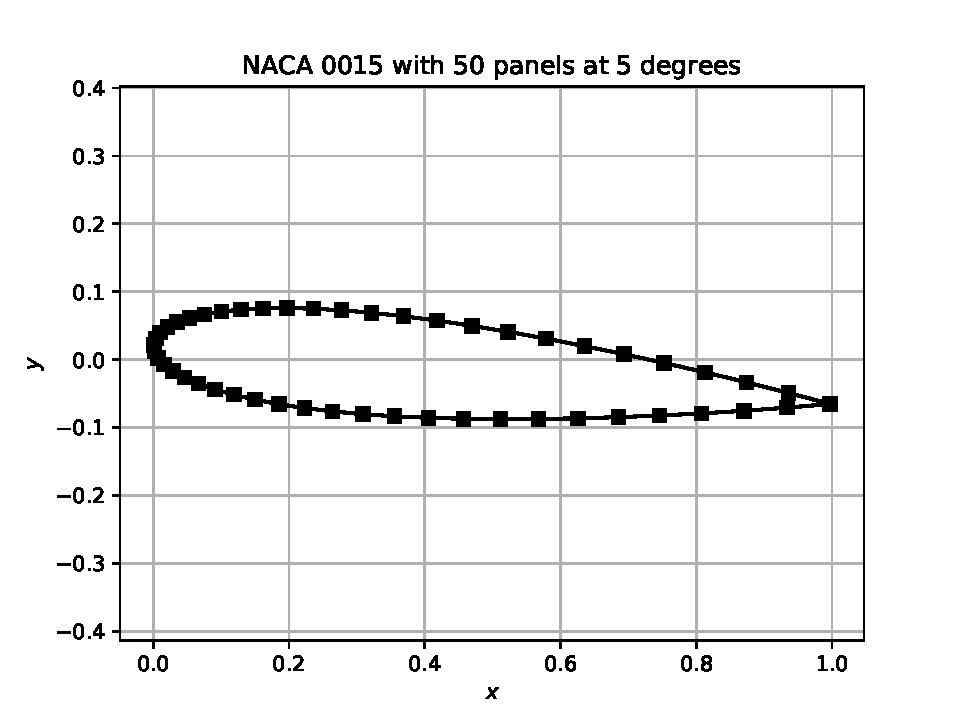
\includegraphics[scale=.5]{plots/naca_panels.pdf}
%\caption{Panel approximation of a NACA airfoil}\label{fig:naca_panels}
%\end{center}
%\end{figure}

To write down the equations, introduce the $N\times N$ influence matrices $B^n$ and $B^t$ such that the influence coefficients $B_{ij}^n$ and $B_{ij}^t$ are the projections onto $\hat{\mathbf n}_i$ and $\hat{\mathbf t}_i$, respectively, of the flow at the $i$th control point (\ie panel midpoint) due to a unit-strength vortex sheet distributed along panel $j$.  That the net flow is tangent at the $i$th control point is expressed by \[A_{i1}^n\sigma_1+\cdots+A_{iN}^n\sigma_N+\gamma\sum_{j=1}^NB_{ij}^n + \mathbf u_\infty\cdot\hat{\mathbf n}_i = 0,\] with one such equation for each panel.  To express the Kutta condition, note that since the airfoil's boundary is a streamline, the Bernoulli equation implies $\frac{1}{2}q_1^2+\frac{p_1}{\rho}=\frac{1}{2}q_N^2+\frac{p_N}{\rho}$, where the subscripts denote control points. The Kutta condition of no trailing-edge loading may be expressed as $p_1=p_N$, which is therefore equivalent to $q_1=q_N$, \ie the flow speed at the upper trailing-edge panel equals that at the lower trailing-edge panel.  Expressing $q_1=q_N$ in terms of the unknowns gives \[A_{11}^t\sigma_1+\cdots+A_{1N}^t\sigma_N+\gamma\sum_{j=1}^NB_{1j}^t+\mathbf u_\infty\cdot\hat{\mathbf t}_1=-\left[A_{N1}^t\sigma_1+\cdots+A_{NN}^t\sigma_N+\gamma\sum_{j=1}^NB_{Nj}^t+\mathbf u_\infty\cdot\hat{\mathbf t}_N\right].\]  The minus sign on the right side arises because the tangent vectors along the airfoil's lower surface are oppositely oriented to the onset flow relative to the tangent vectors along the airfoil's upper surface.  Organizing the $N+1$ equations into matrix-vector form gives \[\begin{bmatrix}A_{11}^n &\cdots &A_{1N}^n &\sum_jB_{1j}^n\\\vdots &\ddots &\vdots &\vdots\\A_{N1}^n &\cdots &A_{NN}^n &\sum_jB_{Nj}^n\\A_{11}^t+A_{N1}^t &\cdots &A_{1N}^t+A_{NN}^t &\sum_jB_{1j}^t+B_{Nj}^t\end{bmatrix}\begin{bmatrix}\sigma_1\\\vdots\\\sigma_N\\\gamma\end{bmatrix} = -\begin{bmatrix}\mathbf u_\infty\cdot\hat{\mathbf n}_1\\\vdots\\\mathbf u_\infty\cdot\hat{\mathbf n}_N\\\mathbf u_\infty\cdot(\hat{\mathbf t}_1+\hat{\mathbf t}_N)\end{bmatrix}.\]  The first $N$ rows of this system are the flow tangency equations, and the last row is the Kutta condition.  After solving this linear system for the unknowns $\sigma_1,\ldots,\sigma_N,\gamma$, the net flow may be computed at any point, from which the pressure distribution may be computed using \eqref{eqn:pressure_coefficient}.  The results of this method applied to a NACA airfoil are shown in \figref{fig:naca_ubem2d}.

\begin{figure}[htbp]
\begin{center}
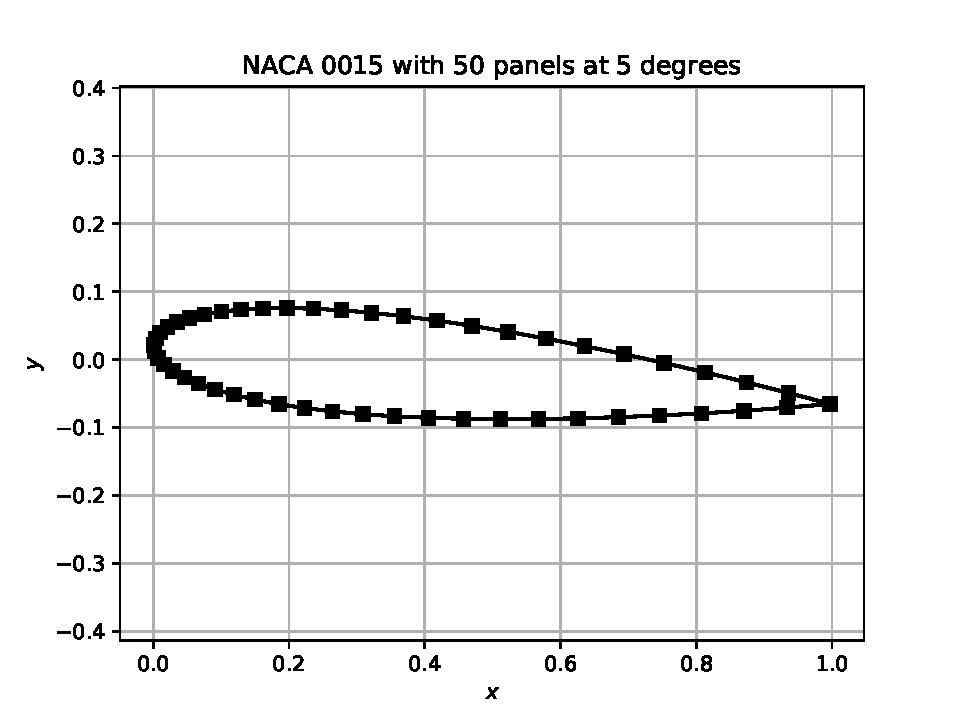
\includegraphics[scale=.4]{plots/naca_panels.pdf}
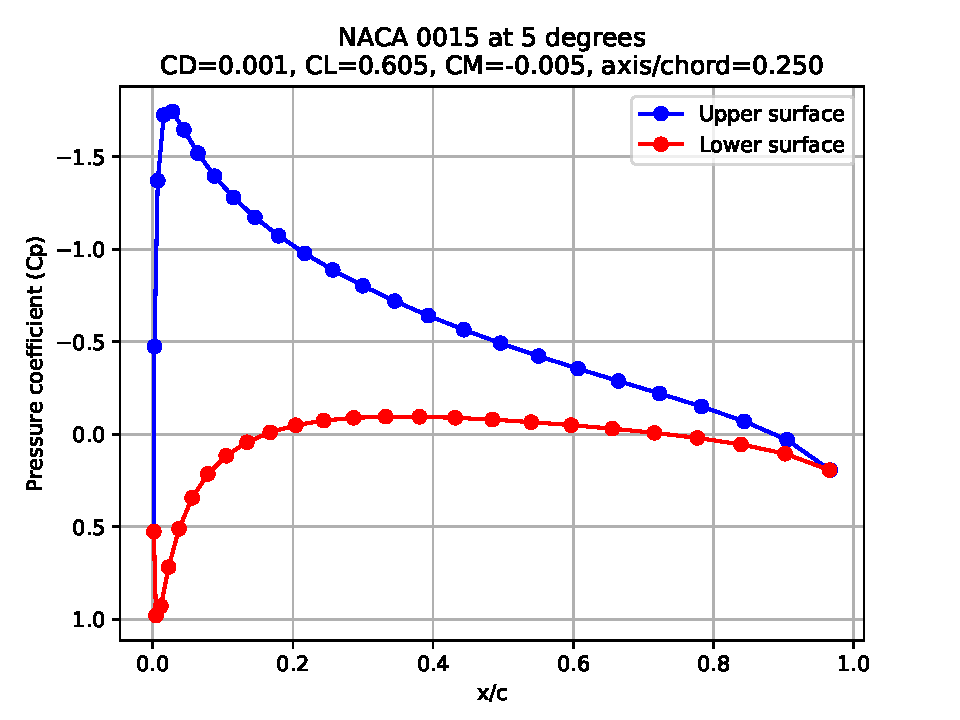
\includegraphics[scale=.4]{plots/naca_cp_boundary.pdf}
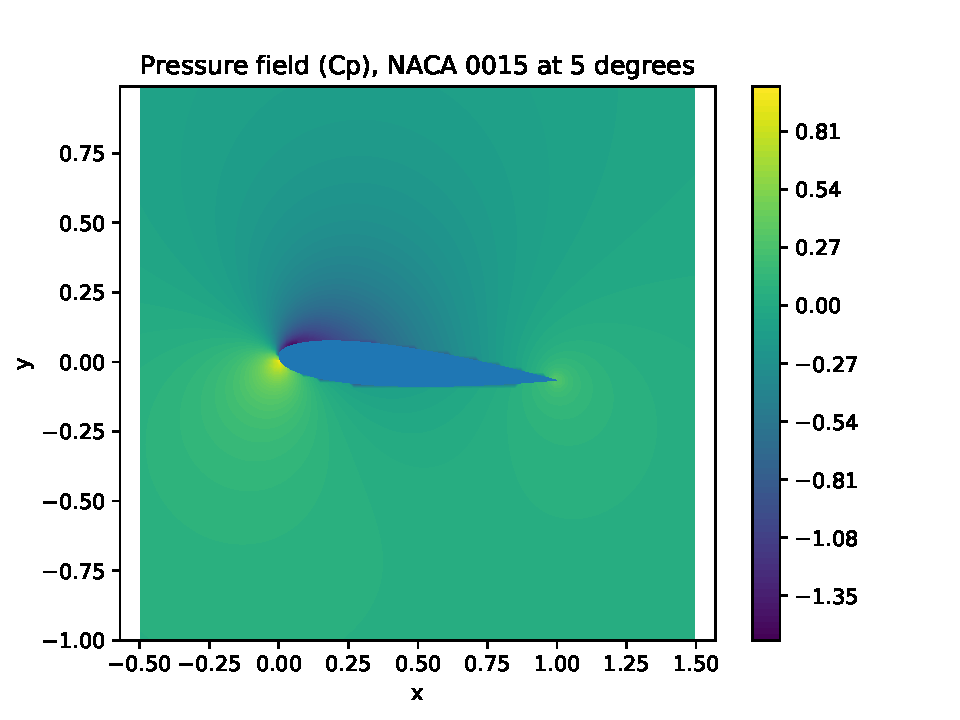
\includegraphics[scale=.4]{plots/naca_cp_field.pdf}
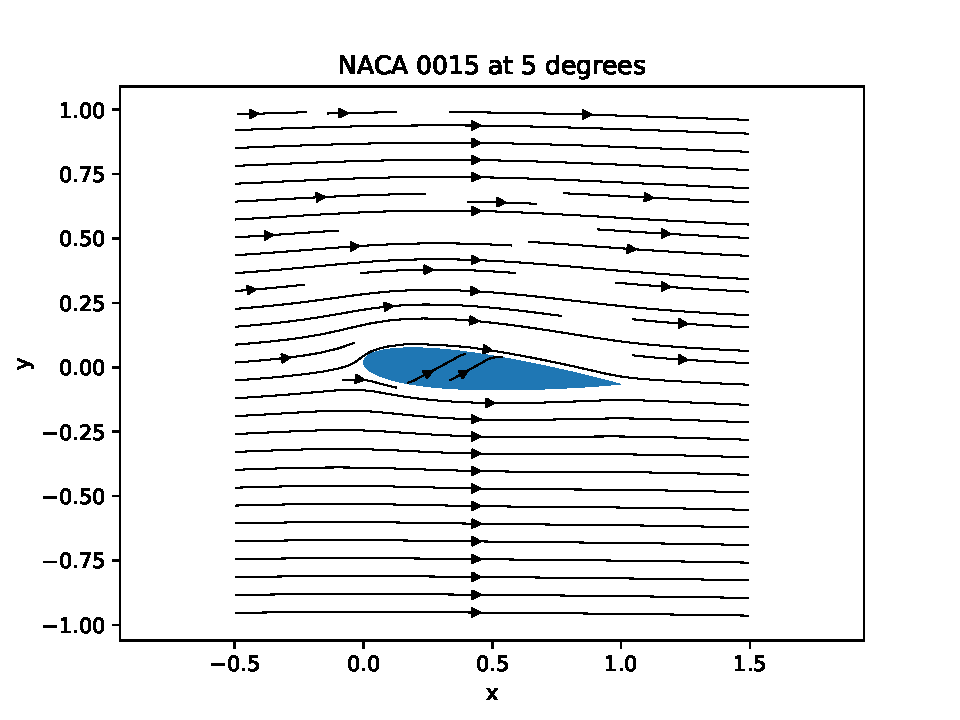
\includegraphics[scale=.4]{plots/naca_streamlines.pdf}
\caption{Results of the Hess-Smith panel method for steady flow $\mathbf u_\infty=\hat{\mathbf x}$ past a NACA airfoil.  Panel corners (upper left), pressure coefficient $C_p$ around the boundary (upper right), pressure distribution in the flow region (lower left), and flow streamlines (lower right).}\label{fig:naca_ubem2d}
\end{center}
\end{figure}

\section{Basu-Hancock method}
We now consider the unsteady flow past a moving airfoil.  The fundamental new feature is the shedding of vorticity into a wake aft of the airfoil.  The basic reason for this is the \defn{Kelvin circulation theorem}, which asserts that the circulation around any closed material curve in the flow of an inviscid incompressible fluid remains constant.  Hence if we consider a large such curve $C$ enclosing the airfoil, then as the airfoil's position and orientation changes relative to the onset flow, the circulation around the airfoil (called the \defn{bound circulation}) must change in order to satisfy the Kutta condition at the trailing edge.  By Kelvin's theorem, this change in bound circulation must be balanced by an equal and opposite change in circulation elsewhere in the fluid contained in $C$.  It is an experimental fact that this balancing circulation is carried in a thin wake which develops aft of the airfoil.

Since the problem is unsteady, we must replace \eqref{eqn:bernoulli_steady} with the \defn{unsteady Bernoulli equation},
\begin{equation}\label{eqn:bernoulli_unsteady}
\pd{\phi}{t} + \frac{1}{2}q^2+\frac{p}{\rho}=\text{constant along a streamline},
\end{equation}
where we make the \defn{quasi-steady} assumption, \ie at each instant in time there exists a scalar potential $\phi$ such that $\mathbf u=\nabla\phi$ holds away in the flow region away from the thin wake.  By similar reasoning as before, the pressure coefficient $C_p$ for unsteady quasi-steady flow is found to be
\[C_p:=\frac{p-p_\infty}{\frac{1}{2}\rho q_\infty^2}=1-\left(\frac{q}{q_\infty}\right)^2-\frac{2}{q_\infty^2}\pd{}{t}(\phi-\phi_\infty).\]
To compute the instantaneous potential $\phi$, we choose a fixed reference point $\mathbf x_\text{ref}$ far upstream of the airfoil.  It then follows from $\mathbf u=\nabla\phi$ that the potential at a field point $\mathbf x$ is
\begin{equation}\label{eqn:potential}
\phi(\mathbf x) = \phi_\infty + \int_{\mathbf x_\text{ref}}^{\mathbf x}\mathbf u\cdot\mathbf{ds},
\end{equation}
where $\phi_\infty$ is the potential at $\mathbf x_\text{ref}$.

We again impose the Kutta condition of no trailing-edge load, \ie $p_1=p_N$, where subscripts denote panel numbers.  It follows from \eqref{eqn:bernoulli_unsteady} that $\pd{\phi_1}{t}+\frac{1}{2}q_1^2+\frac{p_1}{\rho}=\pd{\phi_N}{t}+\frac{1}{2}q_N^2+\frac{p_N}{\rho}$, so that $p_1=p_N$ is equivalent to \[\pd{(\phi_N-\phi_1)}{t}=\frac{1}{2}(q_1^2-q_N^2).\]  Using \eqref{eqn:potential}, we have $\phi_N-\phi_1=\int_1^N\mathbf u\cdot\mathbf{ds}=\gamma L$, where $L$ is the airfoil perimeter.  Note that $\gamma L$ is exactly the instantaneous bound circulation around the airfoil, so that the preceding display may be written \[\pd\gamma t=\frac{q_1^2-q_N^2}{2L}.\]  This is the continuous (or instantaneous) formulation of the Kutta condtion.  We next explain how to set up a discrete simulation.

%If the simulation time step is $\Delta t$ and the circulation at time step $k$ is $\gamma^k$, then we may 

%Next, we need a numerical model of the wake.  As before, the airfoil is partitioned into $N$ panels, along which are placed source sheets of stengths $\sigma_1,\ldots,\sigma_N$, and vortex sheets of common circulation per unit length $\gamma$.

\appendix
\section{Panel integrals and influence coefficients}
To compute the panel influence integrals, \figref{fig:panel_integral} depicts the $j$th body panel, along which is distributed a sheet of singularities of a given type (\eg sources or vortices).  The panel is characterized by its two endpoints, $(x_j,y_j)$ and $(x_{j+1},y_{j+1})$, which determine both the length $L_j$ of the panel and its inclination $\theta_j$ to the positive real axis.  The coordinates of a general point along the panel will be denoted $(\xi,\eta)$.
\begin{figure}[H]
\begin{center}
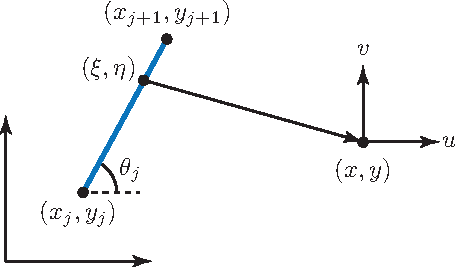
\includegraphics[scale=.8]{figures/panel_integral.pdf}
\caption{Geometry of a panel influence integral}\label{fig:panel_integral}
\end{center}
\end{figure}
The velocity $(u,v)$ at the point $(x,y)$ due to a source distribution of strength $\sigma$ per unit length is given by the path integrals
\begin{align*}
u(x,y)&=\frac{\sigma}{2\pi}\int_0^{L_j}\frac{x-\xi(s)}{(x-\xi(s))^2+(y-\eta(s))^2}\,ds,\\
v(x,y)&=\frac{\sigma}{2\pi}\int_0^{L_j}\frac{y-\eta(s)}{(x-\xi(s))^2+(y-\eta(s))^2}\,ds,
\end{align*}
where $s$ parameterizes arc length along the panel.  By parameterizing the points $(\xi,\eta)$ along the panel by
\begin{equation*}
\begin{aligned}
\xi(s) &:= x_j+s\cos\theta_j,\\
\eta(s) &:= y_j+s\sin\theta_j,
\end{aligned}
\end{equation*}
for $0\leq s\leq L_j$, the integrals become
\begin{align*}
u(x,y) &= \frac{\sigma}{2\pi}\int_0^{L_j}\frac{x-x_j-s\cos\theta_j}{(x-x_j-s\cos\theta_j)^2+(y-y_j-s\sin\theta_j)^2}\,ds\\
v(x,y) &=\frac{\sigma}{2\pi}\int_0^{L_j}\frac{y-y_j-s\sin\theta_j}{(x-x_j-s\cos\theta_j)^2+(y-y_j-s\sin\theta_j)^2}\,ds.
\end{align*}
These integrals are of the general form \[\int_0^{L_j}\frac{\nu s+\mu}{as^2+bs+c}\,ds,\] for appropriately defined constants $\nu,\mu,b,c$ depending only on the panel geometry and the field point, and this integral may be computed by consulting a table of integrals or by using the method of partial fraction expansions as follows:
\paragraph{Case I: $4ac-b^2>0$}
\[\int\frac{\nu s+\mu}{as^2+bs+c}\,ds = \frac{\nu}{2a}\log\left|as^2+bs+c\right|+\frac{2a\mu-b\nu}{a\sqrt{4ac-b^2}}\arctan\frac{2as+b}{\sqrt{4ac-b^2}}+C.\]
\paragraph{Case II: $4ac-b^2=0$}
\[\int\frac{\nu s+\mu}{as^2+bs+c}\,ds = \frac{\nu}{2a}\log\left|as^2+bs+c\right|-\frac{2a\mu-b\nu}{a(2as+b)}+C.\]
\paragraph{Case III: $4ac-b^2<0$}
\[\int\frac{\nu s+\mu}{as^2+bs+c}\,ds = \frac{\nu}{2a}\log\left|as^2+bs+c\right|-\frac{2a\mu-b\nu}{a\sqrt{b^2-4ac}}\text{arctanh}\frac{2as+b}{\sqrt{b^2-4ac}}+C.\]

%For example, assuming $4ac-b^2>0$, both $u(x,y)$ and $v(x,y)$ are given by the expression \[\frac{\sigma}{2\pi}\left[\frac{\nu}{2}\log\left|\frac{L_j^2+bL_j+c}{c}\right|+\frac{2\mu-b\nu}{\sqrt{4c-b^2}}\left(\tan^{-1}\frac{2L_j+b}{\sqrt{4c-b^2}}-\tan^{-1}\frac{b}{\sqrt{4c-b^2}}\right)\right],\] where the values of $\nu,\mu,b,c$ depend on whether one is computing $u(x,y)$ or $v(x,y)$.

Furthermore, when the point $p=(x,y)$ is the panel midpoint, a limiting argument may be used to show that $u(p) = \frac{1}{2}$ and $v(p) = 0$.

\bibliographystyle{alpha}
\bibliography{../bibliography}
\end{document}